\documentclass[tikz,border=6pt]{standalone}
\usepackage{tikz}

\definecolor{paleyellow}{RGB}{255,239,160}
\definecolor{darkyellow}{RGB}{120,90,20}
\definecolor{midblue}{RGB}{120,170,225}
\definecolor{darkblue}{RGB}{20,50,130}

\begin{document}
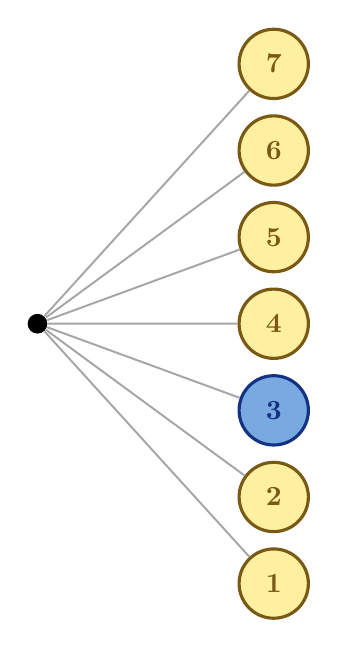
\begin{tikzpicture}[
  yscale=1.1,
  bigcircle/.style={circle, draw=darkyellow, fill=paleyellow, text=darkyellow,
                    minimum size=8.8mm, font=\bfseries, line width=0.4mm,
                    inner sep=0pt},
  bigoptcircle/.style={circle, draw=darkblue, fill=midblue, text=darkblue,
                       minimum size=8.8mm, font=\bfseries, line width=0.4mm,
                       inner sep=0pt},
  dotnode/.style={circle, fill=black, minimum size=2.5mm, inner sep=0pt}
]
  \node[dotnode] (p) at (-3, 4) {};

  \foreach \i in {1,2,4,5,6,7} {
    \node[bigcircle] (c\i) at (0, \i) {\i};
  }
  \node[bigoptcircle] (c3) at (0, 3) {3};

  \foreach \i in {1,...,7} {
    \draw[gray!70, line width=0.25mm] (p) -- (c\i);
  }
\end{tikzpicture}
\end{document}
